\documentclass[10pt]{scrartcl}
\input{eucall_header}

\usepackage{mathtools}
\DeclarePairedDelimiter\ceil{\lceil}{\rceil}
\DeclarePairedDelimiter\floor{\lfloor}{\rfloor}


\ihead{D4.5} % left head

% sophisticated linking of references in the pdf and setting some options
\usepackage{url}                                                  % for correct typesettings of URLs
\usepackage{hyperref}                                             % for sophisticated linking of urls, dois, pictures, tables, etc.
\hypersetup{
    unicode=true,                                                 % non-Latin characters in Acrobat’s bookmarks
    pdftoolbar=true,                                              % show Acrobat’s toolbar?
    pdfmenubar=true,                                              % show Acrobat’s menu?
    pdffitwindow=false,                                           % window fit to page when opened
    pdfstartview={FitH},                                          % fits the width of the page to the window
    pdftitle={D4.5: Testing, validation, and example workflow},   % title
    pdfauthor={C. Fortmann-Grote},                                % author
    pdfsubject={EUCALL WP4 (SIMEX) Deliverable D4.5},             % subject of the document
    pdfcreator={pdflatex},                                        % creator of the document
    pdfnewwindow=true,                                            % links in new PDF window
    colorlinks=true,                                              % false: boxed links; true: colored links
    linkcolor=blue,                                               % color of internal links (change box color with linkbordercolor)
    citecolor=blue,                                               % color of links to bibliography
    filecolor=blue,                                               % color of file links
    urlcolor=blue                                                 % color of external links
}

% Zeilenabstand
\renewcommand{\baselinestretch}{1.2}

\begin{document}
\makeatletter
\begin{titlepage}
\thispagestyle{scrheadings}
\begin{center}
$~$\\
\vspace{0cm}
{\Large\textbf{EUCALL}\\[2ex]
The European Cluster of Advanced Laser Light Sources}\\[4ex]
%
{\small\textbf{Grant Agreement number: 654220}}\\[6ex]
%
Work Package 4 -- SIMEX\\[3ex]
%
Deliverable D4.5\\
%
Testing, validation, and example workflow\\[4ex]
%
Lead Beneficiary: DESY\\[4ex]
%
Carsten Fortmann-Grote,
Johannes Reppin,
Frank Schl\"unzen,
Yves Kempp,
Sergey Yakubov,
Ashutosh Sharma,
Alexander Andreev,
Sakura Pascarelli,
Mathias Sander,
Thomas Kluge,
Marco Garten,
Axel H\"ubl,
Michael Bussmann,
and
Adrian P. Mancuso\\[4ex]
%
Due date: September 30, 2017\\
Delivery date: \today \\[4ex]
%
Project webpage: \url{www.eucall.eu}\\[6ex]
%
{%
\small
\begin{tabular}{|l|l|}
  \hline
  \multicolumn{2}{|l|}{ \textit{Deliverable Type} } \\
  \hline
  R = Report\hfill & R\\
  DEM = Demonstrator, pilot, prototype, plan designs & \\
  DEC = Websites, patents filing, press \& media actions, videos, etc. & \\
  OTHER = Software, technical diagram, etc. & \\
  \hline
  \multicolumn{2}{|l|}{\textit{Dissemination level}} \\
  \hline
  PU = Public, fully open, e.g. web & PU \\
  CO = Confidential, restricted under conditions set out in Model Grant
  Agreement\hspace*{17ex}\  & \\
  CI = Classified, information as referred to in Commission Decision 2001/844/EC
  & \\
  \hline
\end{tabular}
}

\end{center}
%
%\vfill
\centering{%
\includegraphics[width=0.91\textwidth]{figures/PartnerLogos_2017}
}
\normalfont
\end{titlepage}
\makeatother

\section*{Abstract}
%
This report details validation and benchmark studies of the experiment simulation capabilities
developed in EUCALL's workpackage 4 (SIMEX). Where available, we compare our
simulations to experimental data. In other cases, we compare simulations with
simulations, using either different implementations of the same modeling
approach or two simulations of varying degree of accuracy (e.g. 1D vs. 2D
radiation hydrodynamics). The second part contains HPC benchmarks of selected
simulation codes which present performance bottlenecks in the respective
simulation pipeline.
%
\tableofcontents
%
\section{Validation}%
\subsection{Single--particle coherent diffractive imaging\label{sec:single_particle_imaging}}
We present two study cases where we validate and benchmark individual simulation
modules as well as an entire start--to--end simulation toolchain with
experimental data. In the first case, we compare simulated and measured 2D
diffraction data from the Rice Dwarf Virus \cite{Munke2016}, in the second case
we compare 3D molecular structures reconstructed from simulated diffraction data
to the original 3D model reconstructed from NMR \cite{Schlessman1998}
measurements.
\subsubsection{Validation of single--particle imaging using raw diffraction data }
Our validation of the single--particle imaging simulation toolchain in SIMEX
uses diffraction data measured at the AMO endstation at
\SI{1.6}{\kilo\electronvolt} photon energy.
%
\begin{verbatim}
TBC (Carsten)
\end{verbatim}
%
\subsubsection{Validation of the single--particle imaging simulation toolchain
using reconstructed density profiles}%
Coherent diffraction from single proteins has been simulated using the
\textit{simS2E} suite \cite{Yoon2016}. Of the order 200000 diffraction images,
sampling the FEL spectral and temporal fluctuations, including focussing
mirror height profiles, radiation damage processes (ionization and atomic
displacement), were then fed into computational reconstruction using the
Expand--Maximize--Compress (EMC) algorithm for orientation and the
Difference Map (DM) algorithm to solve the phase problem. The resulting 3D
electron density maps could then be compared to the PDB model that was used as
a sample specification in the simulation. The structure in the PDB had been
measured with the NMR method. We reproduce below the corresponding figures
from the original article by Yoon et al.
\begin{figure}[ht]
  \begin{center}
    \includegraphics[width=0.8\textwidth,angle=0,clip]{srep24791-f7}
  \end{center}
  \caption{Electron densities of the average reconstruction at the 5\% and 15\%
    levels (yellow and purple, respectively) from simulated diffraction data with
    (top row) and without (bottom row) Compton scattering and for two different
    XFEL pulse durations. The protein's low--resolution features (original PDB
    shown on left-hand-side) were recovered in
    all four cases, with surface electron densities showing the most variation and
    hence least certainty. Loss of reproducible density is more severe in the
    30 fs case due to greater damage. Degradation of surface contrast is
    expected in
    previous damage--only simulations and may, in future studies, be tampered by a
    sacrificial water layer\cite{Hau-Riege2004}. Reproduced
    from Yoon et al., Scientific Reports \textbf{6}, 24791 (2016) under the
  Creative Commons Attribution 4.0 International License.
}
  \label{fig:2NIP_reconstruction}
\end{figure}
The results demonstrate the predictive power of our start--to--end simulation
toolchain. All main features of the protein were reproduced. Regions close to
the surface show enhanced displacement and poorer agreement with the
experimental data due to radiation damage.
%
\subsection{Coherent Nanocrystal diffraction\label{sec:coherent_nanocrystal_diffraction}}
Two codes integrated in \textit{simex\_platform} can be used to model x--ray
diffraction from crystalline samples. The first code is \textit{singfel},
which calculates the diffraction from given atomic coordinates and scattering
formfactors. The second code is \textit{pattern\_sim} (part of
\textit{crystfel}) \cite{White2012}, which
reads only the crystallographic unit cell and form factors plus information
about the point group and sample size to calculate the diffraction
pattern consisting of Bragg spots and incoherent contributions.
\textit{singfel} reads the structure of the entire nanocrystal, thus providing
more flexibility to account for radiation damage effects which break the
translational symmetry of the sample.

We validate both codes against the code \textit{mercury} \cite{Macrae2008} of the
Cambridge Crystallographic Data Centre (CCDC). Fig.~\ref{fig:Fe2O3_vpp_model_vs_model} shows the simulated
powder diffraction pattern up for \textit{singFEL} vs. \textit{mercury} (top)
and for \textit{pattern\_sim} vs. \textit{mercury} (bottom). The sample is a
\SI{18}{\nano\metre} sized fcc crystal of
Fe\textsubscript{2}O\textsubscript{3}. In both cases, the
positions of Bragg peaks produced by SIMEX correspond to the reference
simulation. In general, the peak amplitudes differ between the SIMEX simulations and the
reference model, while the \textit{singFEL} results are in better agreement to the
reference model than the \textit{pattern\_sim} results. This difference between
\textit{singFEL} and \textit{pattern\_sim} can be attributed to the more
precise and well validated model for the form factors, calculated with the code \textit{XATOM}
\cite{Son2011}. Note that the \textit{singFEL} calculation contains a
large signal at small angles, this has been removed in the \textit{pattern\_sim}
calculation. These simulations were used to support the feasibility of a
experiment proposed at European XFEL.
%
\begin{figure}[ht]
  \begin{center}
      \includegraphics[width=.8\textwidth,angle=0,clip]{Fe2O3_vpp_mercury_vs_simex}
      \includegraphics[width=.8\textwidth,angle=0,clip]{Fe2O3_vpp_mercury_vs_patternsim}
  \caption{Simulated powder diffraction patterns (blue lines) for nanocrystalline fcc Fe\textsubscript{2}O\textsubscript{3}
  using the diffraction modules \textit{singfel} (top) and \textit{pattern\_sim}
  (bottom) compared to reference calculations for an infinite fcc lattice
    using the code \textit{mercury} (orange curve).}
    \label{fig:Fe2O3_vpp_model_vs_model}
  \end{center}
\end{figure}
%

In the following, we will
apply the \textit{singFEL} module for diffraction simulations and compare to
experimental data.
Fig.~\ref{fig:C60_virtual_powder_data_vs_models} compares \textit{singfel}
simulations to diffraction data from
an experiment at the CXI endstation at LCLS in a virtual powder representation.
The sample is fcc nanocrystalline C\textsubscript{60}. Bragg peaks were identified in each measured
2D diffraction pattern using the \textit{psana} \cite{psana_www} peak finder
and histogrammed according to the peak's
radial distance from the geometrical center of the detector image corresponding
to zero scattering angle.
The histogram (orange bars) is plotted as a function of the Bragg
angle $2\theta$ and compared to a SIMEX simulation using \textit{singfel}
(blue curve) and the \textit{mercury} reference calculation for a perfect
infinite fcc lattice. Similar to the model--vs--model comparison, the agreement
between models and data is overall satisfying, i.e. the peak positions coincide
and the peak amplitudes are close.
%
\begin{figure}[ht]
  \begin{center}
    \includegraphics[width=.8\textwidth,angle=0,clip]{C60_Abbey2016_phaseAfcc_lowFluence_vs_simex_noRD}
  \end{center}
  \caption{Virtual powder pattern from nanocrystalline C\textsubscript{60}
  \cite{Abbey2016} (orange curve) compared to SIMEX
  simulations for a 10x10x10 C\textsubscript{60} fcc supercell using the code
  \textit{pysingfel} (blue curve) and compared to a modeled powder pattern for
  an infinite C\textsubscript{60} fcc lattice using the code \textit{mercury}.}
  \label{fig:C60_virtual_powder_data_vs_models}
\end{figure}
%
\subsection{Imaging of High--Power Laser driven targets\label{sec:high_power_imaging}}
\begin{verbatim} TODO: HZDR \end{verbatim}
%
\subsection{Liquid jet crystal diffraction\label{sec:liquid_crystals}}
\begin{verbatim} TODO: Mathias (ESRF) \end{verbatim}
%
\subsection{Warm dense matter x--ray absorption spectroscopy\label{sec:warm_dense_matter_spectroscopy}}
Interaction of high--energy optical laser pulses with solid targets and shock
compression is modeled with radiation--hydrodynamics (RH) simulations using
either 1D (\textit{Esther} \cite{Colombier2005})
or 2D (\textit{Multi2D} \cite{Ramis2009}) RH implementations.
The resulting profiles for mass density, temperature,
ionization, and pressure are then fed into an electronic structure calculation.
Finally, a real--space Green function code (e.g. FEFF \cite{Rehr2009} calculates the x--ray absorption
spectrum. At this point, the spectrum and intensity distribution of the x--ray
probe beam, delivered by x--ray raytracing simulations can be taken into
account. The workflow, supported by SIMEX is shown in
Fig.~\ref{fig:xas_workflow}.
%
\begin{figure}[ht]
  \begin{center}
    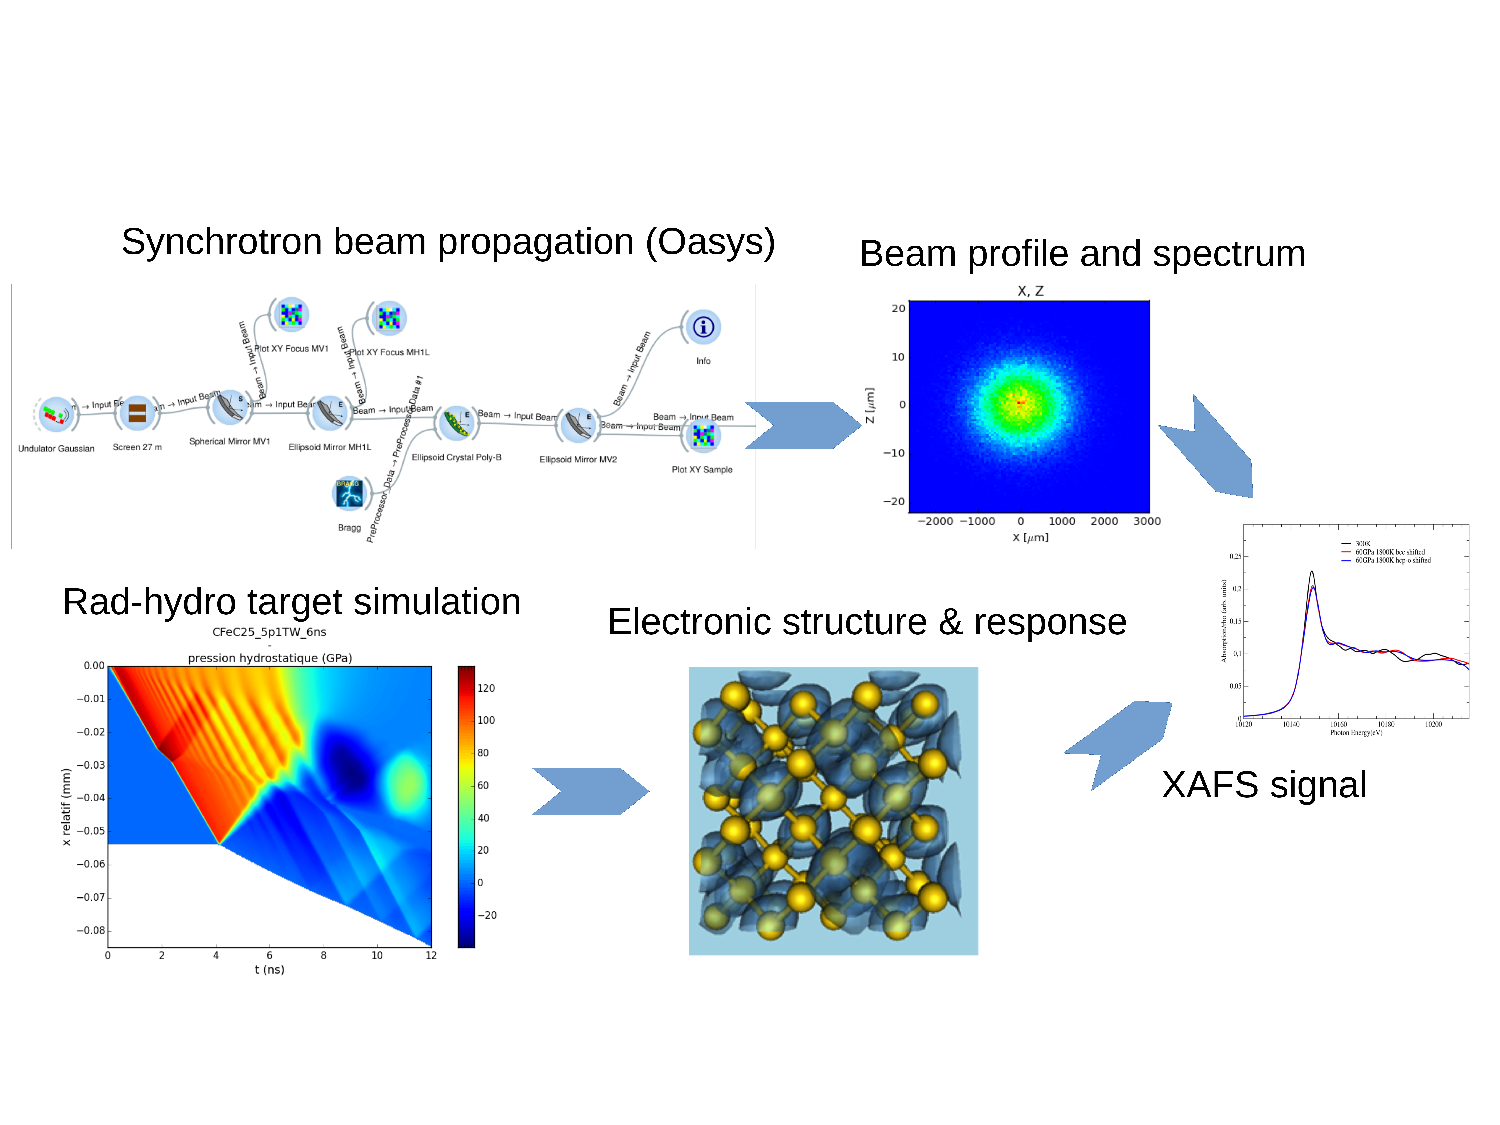
\includegraphics[width=0.8\textwidth,angle=0,clip]{simex_xas_workflow}
  \end{center}
  \caption{SIMEX workflow for simulations of x--ray absorption spectroscopy of
  shock--compressed warm dense matter generated by high--energy long pulse laser
--matter interaction.}
  \label{fig:xas_workflow}
\end{figure}
%
Fig.~\ref{fig:xas_setup_rh} shows details on the experiment carried out at
beamline ID24 at ESRF against which we validate our simulations.
%
\begin{figure}[ht]
  \begin{center}
    \includegraphics[width=0.8\textwidth,angle=0,clip]{torchio2016}
  \end{center}
  \caption{Target geometry (a), experimental setup (b), and XANES spectra (c)
    from ESRF ID24 experiment as reported in [Torchio et al. Scientific Reports \textbf{6}, 26402
    (2016)], 1D
  (d) and 2D (e) radiation--hydrodynamics simulation of the laser--matter
interaction.}
  \label{fig:xas_setup_rh}
\end{figure}
%
\begin{figure}[ht]
  \begin{center}
    \includegraphics[width=0.8\textwidth,angle=0,clip]{xas_exp_vs_AI.jpg}
  \end{center}
  \caption{Left: Experimental EXAFS spectra close to the K--edge at two different pressure and temperature conditions realized
    in the experiment compared to ambient conditions (black line). Right: ab-initio
  molecular dynamic simulations. Labels a,b,c,d mark points in the spectrum where
  strong deviations from the ambient spectrum is observed as indicated by black
  arrows. These are
  qualitatively reproduced in the ab--initio simulations.
  Figure reproduced from [Torchio et al. Scientific Reports \textbf{6}, 26402
    (2016)] under Creative Commons Attribution 4.0 International License.}
  \label{fig:xas_exp_vs_AI}
\end{figure}
%
In Fig.~\ref{fig:xas_exp_vs_AI}, we show experimental EXAFS
spectra, measured at beamline ID24 at ESRF \cite{Torchio2016} compared to ab--initio
simulations assuming pressure and temperature conditions similar to those of
the experiment, which were modelled with RH simulations. The experimental spectra
measured at \SI{500}{\giga\pascal} pressure and \SI{1.7e4}{\kelvin} temperature
(upper left) and at \SI{120}{\giga\pascal} pressure and \SI{2.7e3}{\kelvin}
temperature (lower left), respectively, are shown in together with spectra
measured at ambient conditions (black curve). The labels a,b,c, and d mark points
in the spectrum, where the strongly compressed case shows significant
differences with respect to the ambient case. At increased pressure, a shift of
the K--edge onset to smaller energie is found, as well as a steepening of the
edge profile in the lower half of the edge retion
(\SI{<7.12}{\kilo\electronvolt}), whereas the absorption rises less steeply with respect to the
ambient case in the upper half of the edge (\SI{>7.12}{\kilo\electronvolt}).
The modelled spectra reproduce
these differences qualitatively. A more quantitative analysis and comparison
beteen theory and experiment is still outstanding.
%

We also compared 1D RH simulations for the (peak??) pressure as a function
of energy on target in the case of molybdenum. Fig.~\ref{fig:rh_1d_vs_exp}
shows three measured datasets (dots) differing the the thickness of the phase plate
used to smoothen the intensity distribution over the focal spot and the pump
pulse duration. The solid lines mark the RH simulations, systematically
overestimating the pressure. This is a typical artifact of 1D RH simulations.
The systematic offset between model and data could be used to define a heuristic
correction factor to apply to 1D simulation data.
%
\begin{figure}[ht]
  \begin{center}
    \includegraphics[width=.8\textwidth,angle=0,clip]{RadHydro_Mo_1D_vs_exp}
  \end{center}
  \caption{Pressure vs. energy on target (molybdenum) for three different phase plate
  thicknesses and pulse durations. The 1D radiation--hydrodynamics simulations
  (solid lines) systematically overestimate the experimental conditions (dots).}
  \label{fig:rh_1d_vs_exp}
\end{figure}

\subsection{Wavefront propagation through phase gratings}
\label{sec:wpg_phasegrating}
\begin{verbatim}
TODO L. Mikes.
\end{verbatim}
%
\FloatBarrier
%
\section{High Performance Computing Benchmarks}
\subsection{Single--particle imaging simulation pipeline}
The single--particle imaging simulatoin pipeline consists of
\begin{enumerate}
  \item pulse propagation
  \item photon--matter interaction
  \item diffraction
  \item detector response (optional)
\end{enumerate}

Each of these modules have very different and demanding computational resource
requirements. We present benchmarking results for few selected modules which
represent performance bottlenecks in the simulation pipeline.

\subsubsection{Wavefront propagation}
The wavefront propagation utilizes the software Synchrotron Radiation Workshop
(SRW), a legacy C library with historically very limited options for
parallelization. Recently, there have been three major developments:
\begin{enumerate}
  \item Insertion of openMP macros to enable shared--memory parallelism
  \item Multicore parallel execution of propagation of multiple FEL source
    pulses.
  \item MPI parallel calculation of independent coherent modes for partially
    coherent wavefront propagation.
\end{enumerate}
%
1) and 2) have been realized in SIMEX, 3) is an independent development in the radiation source
simulation and propagation framework SiRepo
\url{www.github.com/radiasoft/sirepo}. Fig.~\ref{fig:srw_speedup} shows the
speedup of a single SRW wavefront propagation resulting from the insertion of
openMP pragmas in the SRW source code.
%
\begin{figure}[ht]
  \begin{center}
    \includegraphics[width=0.8\textwidth,angle=0,clip]{srw_speedup-crop}
  \end{center}
  \caption{Speedup of WPG/SRW wavefront propagation for a single source input
  file using openMP shared--memory parallelism.}
  \label{fig:srw_speedup}
\end{figure}
%
\begin{table}
  \centering
  \begin{tabular}{rrrr}
    \textbf{Threads x MPI processes} & \textbf{Number of nodes} &
    \textbf{Wall time (min)} & \textbf{Time/input file (s)} \\
    \hline
    1x1        & 1     & 660       &  1031 \\
    40x1       & 1     &  65       &    98 \\
    4x10       & 4     &   7.5     &    45 \\
    8x5        & 8     &   4.2     &    51 \\
  \end{tabular}
  \caption{Total wall time  taken by the propagation of 40 individual source files with hybrid
  openMP/MPI parallelism in SRW. Note how the distribution of MPI processes over nodes
and threads influences the walltime and the time to process each file.}
  \label{tab:srw_hybrid_timings}
\end{table}
%
\subsubsection{Radiation damage}
The radiation damage module is by far the most compute intensive part of the SPI
pipeline, determining $\approx 90\%$ of the total wall time of one
start--to--end propagation. The code \textit{xmdyn and xatom}, provided by
CFEL, DESY \cite{Jurek2016} utilizes GPGPU cards, MPI or shared memory
parallelism are currently not implemented, only one GPGPU card can
be utilized at a time. Our benchmarks therefore compare the performance on
different GPGPU variants. The test case is a trajectory of the 2NIP protein
irradiated by a \SI{10}{\femto\second} (FWHM) pulse of
\SI{5}{\kilo\electronvolt} FEL photons (pulse energy \SI{\approx 1}{\milli\joule}).
%
\begin{table}
  \centering
  \begin{tabular}{rrr}
    \textbf{GPU model} & \textbf{Total wall time first run (s)} & \textbf{Total
    wall time subseq. run (s)}\\
    \hline
    K20X  & 580 & 568 \\
    K40X  & 484 & 470 \\
    P100  & 470 & 466 \\
  \end{tabular}
  \caption{Wall time for a single \textit{xmdyn and xatom} run on different
NVIDIA(C) GPGPU car. The first run take longer because the atomic transition database
has to be populated.}
  \label{tab:xmdyn_performance_nvidia}
\end{table}
%
\subsubsection{Diffraction}
%
Diffraction calculations are performed with the code \textit{pysingfel}. To
enhance performance, this code uses the \textit{numba} library to facilitate
just--in--time compilation for available hardware of compute intensive parts.
In the following we benchmark the performance of a \textit{pysingfel} diffraction
calculation with an unperturbed protein diffracting a parametrized FEL beam of
\SI{5}{\kilo\electronvolt} photon energy into a detector of 1024x1024 pixels.
%%%%%%%%%%%%%%%%%%%%%%%%%%%
\printbibliography[title={References}]
%
%\printbibliography[keyword=submitted, title={Submitted articles}]
%
%\printbibliography[keyword=inpreparation, title={Articles in preparation}]
%
%\printbibliography[keyword=eucall, keyword=report, title={Project reports}]
%

%%%%%%%%%%%%%%%%%%%%%%%%%%%
\end{document}


